\part En el momento que sigue en la simulación, la porción de la energía cinética de la gráfica circular crece, entonces:

\begin{minipage}{0.3\textwidth}
    \begin{figure}[H]
        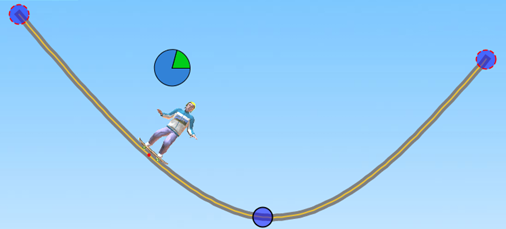
\includegraphics[width=\linewidth]{../images/q028c}
    \end{figure}
\end{minipage}\hfill
\begin{minipage}{0.6\textwidth}
    \begin{choices}
        \choice El patinador va hacia arriba en la pista (hacia la izquierda)
        \choice El patinador va hacia abajo en la pista (hacia la derecha)
        \choice No hay manera de saberlo
    \end{choices}
\end{minipage}
